\documentclass[12pt]{article}

\usepackage{sbc-template}
\usepackage{graphicx,url}
\usepackage[utf8]{inputenc}
\usepackage[T1]{fontenc}
\usepackage[brazil]{babel}
\usepackage{amsmath}
\usepackage{booktabs}
\usepackage{tikz}
\usetikzlibrary{arrows.meta,positioning}

\graphicspath{{figuras/}{../reports/figures/}}
\sloppy

% TODO: preencher título final, autores e e-mails.
\title{Predição de risco de insuficiência cardíaca com aprendizado de máquina:\\
comparação de modelos e aplicação web de triagem}

\author{Nome do Autor 1\inst{1}, Nome do Autor 2\inst{1}}

\address{Curso de Ciência da Computação -- Universidade Federal do Maranhão (UFMA)\\
  São Luís -- MA -- Brasil
  \email{\{autor1,autor2\}@discente.ufma.br}
}

\begin{document}

\maketitle

\begin{abstract}
  Cardiovascular diseases are the leading cause of death worldwide, and heart
  disease is the main precursor of heart failure, which makes early detection
  essential. This work evaluates machine learning classifiers that estimate the
  risk of heart disease from 11 routine clinical attributes. Seven approaches
  are compared on a public dataset of 918 patients, under a leakage-free
  protocol with a stratified hold-out and repeated cross-validation. The
  selected Random Forest obtained an AUC-ROC of 0.923 on the test set and, with
  a decision threshold adjusted for sensitivity, a recall of 0.951 and a
  precision of 0.782. The model was integrated into a web application that
  validates inputs, reports the probability and explains each prediction.
\end{abstract}

\begin{resumo}
  As doenças cardiovasculares são a principal causa de morte no mundo, e a
  doença cardíaca é o principal precursor da insuficiência cardíaca, o que
  torna essencial a detecção precoce. Este trabalho avalia classificadores de
  aprendizado de máquina que estimam o risco de doença cardíaca a partir de 11
  atributos clínicos de rotina. São comparadas sete abordagens em um conjunto
  público com 918 pacientes, sob protocolo sem vazamento de dados. O Random
  Forest selecionado obteve AUC-ROC de 0,923 no teste e, com o limiar ajustado
  para sensibilidade, revocação de 0,951 e precisão de 0,782. O modelo foi
  integrado a uma aplicação web que valida as entradas, informa a
  probabilidade e explica cada predição.
\end{resumo}

\section{Introdução}
\label{sec:introducao}

As doenças cardiovasculares constituem a principal causa de morte no mundo.
Estimativas da Organização Mundial da Saúde indicam que 19,8 milhões de pessoas
morreram por essas doenças em 2022, o que corresponde a cerca de 32\% de todas
as mortes, e que mais de três quartos desses óbitos ocorreram em países de
baixa e média renda \cite{who:25}. No Brasil, elas respondem por perto de um
terço das mortes e atingem de forma desproporcional a população mais pobre
\cite{oliveira:24}.

A insuficiência cardíaca é o desfecho comum de várias dessas doenças, em
especial da doença arterial coronariana. Desta forma, a detecção precoce
torna-se o principal recurso para iniciar o tratamento antes do agravamento
do quadro \cite{who:25}. O diagnóstico definitivo, contudo, exige exames
caros ou invasivos, enquanto dados demográficos, exames laboratoriais simples
e o teste de esforço são mais acessíveis. Nesse contexto, métodos de
aprendizado de máquina vêm sendo investigados como apoio à triagem, por
fornecerem uma segunda opinião ao profissional de saúde.

Os trabalhos que seguem essa abordagem reportam acurácias entre 87\% e 100\%
\cite{amin:19,mohan:19,ali:21}. Esses resultados, contudo, costumam ser
apresentados como um único número, sem medida de dispersão nem indicação do
tipo de erro cometido. Além disso, os valores ausentes registrados como zero
nas bases públicas raramente são discutidos, e os modelos não chegam a ser
entregues em uma ferramenta utilizável.

Assim, este trabalho tem como objetivo avaliar classificadores que estimam, a
partir de 11 atributos clínicos de rotina, a probabilidade de um paciente
apresentar doença cardíaca, e integrar o modelo selecionado a uma aplicação
web de apoio à triagem. As principais contribuições são: (a) uma comparação
de sete abordagens, de cinco famílias de algoritmos, sob protocolo
reprodutível e sem vazamento de dados; (b) uma análise de qualidade dos dados
que identifica um viés de coleta no atributo colesterol e mede o seu efeito;
(c) a interpretação do modelo final por importância por permutação, valores
SHAP, subgrupos e análise de erros; e (d) uma aplicação que carrega o
\textit{pipeline} treinado, valida as entradas e explica cada predição. O
código está disponível em repositório público\footnote{% TODO: substituir pelo link real do repositório
\url{https://github.com/USUARIO/predicao-insuficiencia-cardiaca}}.

O restante deste artigo está organizado da seguinte forma. As
Seções~\ref{sec:fundamentacao} e~\ref{sec:relacionados} apresentam a
fundamentação teórica e os trabalhos relacionados. A
Seção~\ref{sec:metodologia} descreve a metodologia. As
Seções~\ref{sec:resultados} e~\ref{sec:aplicacao} apresentam os resultados e
a aplicação. Por fim, as Seções~\ref{sec:etica} e~\ref{sec:conclusao} trazem
as considerações éticas e a conclusão.

\section{Fundamentação teórica}
\label{sec:fundamentacao}

Esta seção apresenta os algoritmos de classificação e as métricas utilizados
neste trabalho. Na classificação supervisionada, busca-se uma função que
estime $P(y=1 \mid x)$ a partir de exemplos rotulados. A regressão logística modela o logaritmo da razão de chances como combinação
linear dos atributos. O k-NN classifica pelo voto dos $k$ vizinhos mais
próximos no espaço de atributos. A máquina de vetores de
suporte (SVM) procura o hiperplano de margem máxima e, com um núcleo como o
RBF, produz fronteiras não lineares \cite{cortes:95}. O Random Forest agrega
árvores de decisão treinadas em amostras \textit{bootstrap}, com sorteio de
atributos em cada divisão, o que reduz a variância \cite{breiman:01}. O
Gradient Boosting soma árvores rasas em sequência, cada uma ajustada ao
gradiente do erro das anteriores \cite{friedman:01}. Por fim, o perceptron
multicamadas (MLP) é uma rede neural de camadas densas treinada por
retropropagação.

Para a avaliação, consideram-se as contagens de verdadeiros positivos (VP),
falsos positivos (FP) e falsos negativos (FN). A precisão é dada por
$\mathrm{VP}/(\mathrm{VP}+\mathrm{FP})$, e a revocação, ou sensibilidade, por
$\mathrm{VP}/(\mathrm{VP}+\mathrm{FN})$. A medida $F_\beta$
(Equação~\ref{eq:fbeta}) combina as duas:
\begin{equation}
\label{eq:fbeta}
F_\beta = (1+\beta^2)\,\frac{\text{precisão}\cdot\text{revocação}}
{\beta^2\,\text{precisão}+\text{revocação}},
\end{equation}
em que $\beta=1$ resulta no F1 e $\beta=2$ atribui à revocação o dobro do
peso. A curva ROC relaciona a taxa de verdadeiros positivos à de falsos
positivos em todos os limiares de decisão, e a área sob ela (AUC-ROC)
corresponde à probabilidade de o modelo atribuir pontuação maior a um doente
do que a um saudável escolhidos ao acaso.

Para a interpretação, a importância por permutação mede quanto uma métrica
piora quando os valores de um atributo são embaralhados \cite{breiman:01}. Os
valores SHAP, por sua vez, distribuem entre os atributos a diferença entre a
predição de um paciente e a predição média \cite{lundberg:17}.

\section{Trabalhos relacionados}
\label{sec:relacionados}

Esta seção apresenta trabalhos disponíveis na literatura que utilizaram dados
clínicos tabulares na predição de doenças cardíacas. As bases empregadas na
maioria deles derivam das coletadas por \cite{detrano:89}, que avaliaram uma
função discriminante em três grupos externos de pacientes e observaram que o
algoritmo superestimava a probabilidade de doença em dois deles.

\cite{amin:19} compararam sete técnicas de classificação sobre subconjuntos
de atributos das bases do UCI e obtiveram 87,4\% de acurácia com um voto
entre Naive Bayes e regressão logística. Na base de Cleveland,
\cite{mohan:19} propuseram um modelo híbrido de Random Forest com modelo
linear (HRFLM), com acurácia de 88,7\%. Já \cite{ali:21} avaliaram k-NN,
árvore de decisão e Random Forest em uma base do Kaggle e relataram 100\% de
acurácia com o Random Forest.

Mais recentemente, \cite{chulde:25} compararam cinco classificadores em uma
base do Kaggle com 918 registros que, pela descrição, é a mesma deste
trabalho, e obtiveram AUC de 0,97 com o Random Forest.

A Tabela~\ref{tab:relacionados} resume esses trabalhos. Em síntese, a
literatura concentra-se na acurácia agregada, obtida sob protocolos distintos,
de modo que os valores não são diretamente comparáveis. Diferentemente desses
trabalhos, o presente estudo reporta média e desvio-padrão em validação
cruzada e intervalos de confiança no teste, trata os valores ausentes
codificados como zero e entrega o modelo em uma aplicação.

\begin{table}[!htb]
\centering
\caption{Trabalhos relacionados. Os resultados são os reportados pelos próprios
autores, sob protocolos distintos.}
\label{tab:relacionados}
\footnotesize
\begin{tabular}{@{}p{4.45cm}p{2.75cm}p{3.1cm}p{3.0cm}@{}}
\toprule
Trabalho & Dados & Técnicas & Melhor resultado reportado \\
\midrule
\cite{detrano:89} & Três grupos externos de pacientes & Função discriminante & Superestima o risco em dois dos grupos \\
\cite{amin:19} & UCI Heart Disease (Cleveland e Statlog) & k-NN, árvore, NB, RL, SVM, rede neural, voto & Voto: acurácia 87,4\% \\
\cite{mohan:19} & UCI Heart Disease (Cleveland) & Híbrido HRFLM e outros & HRFLM: acurácia 88,7\% \\
\cite{ali:21} & Base de doença cardíaca do Kaggle & k-NN, árvore, Random Forest & Random Forest: acurácia 100\% \\
\cite{chulde:25} & Base do Kaggle com 918 registros & RL, RF, árvore, k-NN, MLP & Random Forest: AUC 0,97 \\
\midrule
Este trabalho & 918 pacientes, 11 atributos & 7 abordagens, 5 famílias & Random Forest: AUC 0,923; revocação 0,951 \\
\bottomrule
\end{tabular}
\end{table}

\section{Metodologia}
\label{sec:metodologia}

Esta seção descreve os materiais e o método utilizados no trabalho. O método
está organizado em cinco etapas (Figura~\ref{fig:etapas}): (1) aquisição dos
dados e formulação do problema, (2) análise exploratória, (3)
pré-processamento, (4) treinamento e seleção dos modelos e (5) avaliação e
interpretação. Os experimentos são implementados em Python 3.11 com a
biblioteca scikit-learn \cite{pedregosa:11}, com semente aleatória fixada em
42.

\begin{figure}[!htb]
\centering
\scriptsize
\begin{tikzpicture}[
  node distance=4mm,
  etapa/.style={draw, rounded corners=2pt, align=center, inner sep=2.5pt, minimum height=7mm, text width=2.3cm},
  arr/.style={-{Stealth[length=2mm]}, thick}]
\node[etapa] (e1) {(1) Aquisição dos dados e formulação};
\node[etapa, right=of e1] (e2) {(2) Análise exploratória};
\node[etapa, right=of e2] (e3) {(3) Pré-processamento};
\node[etapa, right=of e3] (e4) {(4) Treinamento e seleção};
\node[etapa, right=of e4] (e5) {(5) Avaliação e interpretação};
\draw[arr] (e1) -- (e2);
\draw[arr] (e2) -- (e3);
\draw[arr] (e3) -- (e4);
\draw[arr] (e4) -- (e5);
\end{tikzpicture}
\caption{Etapas da metodologia.}
\label{fig:etapas}
\end{figure}

\subsection{Aquisição dos dados e formulação do problema}

Este estudo utiliza o \textit{Heart Failure Prediction Dataset}
\cite{fedesoriano:21}, base pública distribuída sob a licença Open Database
License, com o conteúdo pertencente aos autores originais. A base reúne cinco
conjuntos do repositório UCI \cite{janosi:89} e totaliza 918 pacientes após a
remoção de duplicatas. Como não há nomes, documentos ou outros
identificadores, os dados estão anonimizados nos termos da LGPD
\cite{lgpd:18}.

O problema é formulado como uma tarefa de classificação binária. A
variável-alvo é \texttt{HeartDisease}, em que 1 indica doença cardíaca
diagnosticada e 0, ausência. A base é apresentada por seu autor como voltada
à predição de insuficiência cardíaca, por ser a doença cardíaca o seu
principal precursor; neste trabalho, prediz-se a presença de doença cardíaca,
utilizada como indicador desse risco. A Tabela~\ref{tab:dicionario} apresenta
os 11 atributos de entrada.

\begin{table}[!htb]
\centering
\caption{Dicionário de dados dos atributos de entrada.}
\label{tab:dicionario}
\footnotesize
\begin{tabular}{@{}llll@{}}
\toprule
Atributo & Descrição & Tipo & Valores \\
\midrule
Age & Idade & numérico & 28 a 77 anos \\
Sex & Sexo & categórico & M, F \\
ChestPainType & Tipo de dor no peito & categórico & ASY, ATA, NAP, TA \\
RestingBP & Pressão arterial em repouso & numérico & 0 a 200 mm Hg (1 zero) \\
Cholesterol & Colesterol sérico & numérico & 0 a 603 mg/dl (172 zeros) \\
FastingBS & Glicemia de jejum $>$ 120 mg/dl & binário & 0, 1 \\
RestingECG & ECG em repouso & categórico & Normal, ST, LVH \\
MaxHR & Frequência cardíaca máxima no esforço & numérico & 60 a 202 bpm \\
ExerciseAngina & Angina induzida por exercício & categórico & N, Y \\
Oldpeak & Depressão de ST no esforço & numérico & $-$2,6 a 6,2 mm \\
ST\_Slope & Inclinação do segmento ST no esforço & categórico & Up, Flat, Down \\
\bottomrule
\end{tabular}
\end{table}

Quanto à métrica de sucesso, considera-se que, em triagem, deixar de
encaminhar um doente (falso negativo) é mais grave do que encaminhar um
saudável (falso positivo). Por esse motivo, a revocação é adotada como
métrica de domínio. Como ela depende do limiar e chega a 1 em um modelo que
marca todos como doentes, a seleção de hiperparâmetros e de modelo é
conduzida pela AUC-ROC, e o limiar é definido pela maximização de $F_2$.

\subsection{Análise exploratória}

Nesta etapa, examinam-se a estrutura e a qualidade dos dados no conjunto
completo, e as relações entre atributos e alvo apenas no conjunto de treino,
para que nenhuma decisão dependa do teste. As classes são levemente
desbalanceadas, com 508 pacientes (55,3\%) com doença cardíaca e 410
(44,7\%) sem (Figura~\ref{fig:alvo}a). A distribuição por sexo, por outro
lado, é desigual (Figura~\ref{fig:alvo}b): 79\% dos registros são de homens,
e apenas 50 mulheres apresentam o desfecho positivo.

\begin{figure}[!htb]
\centering
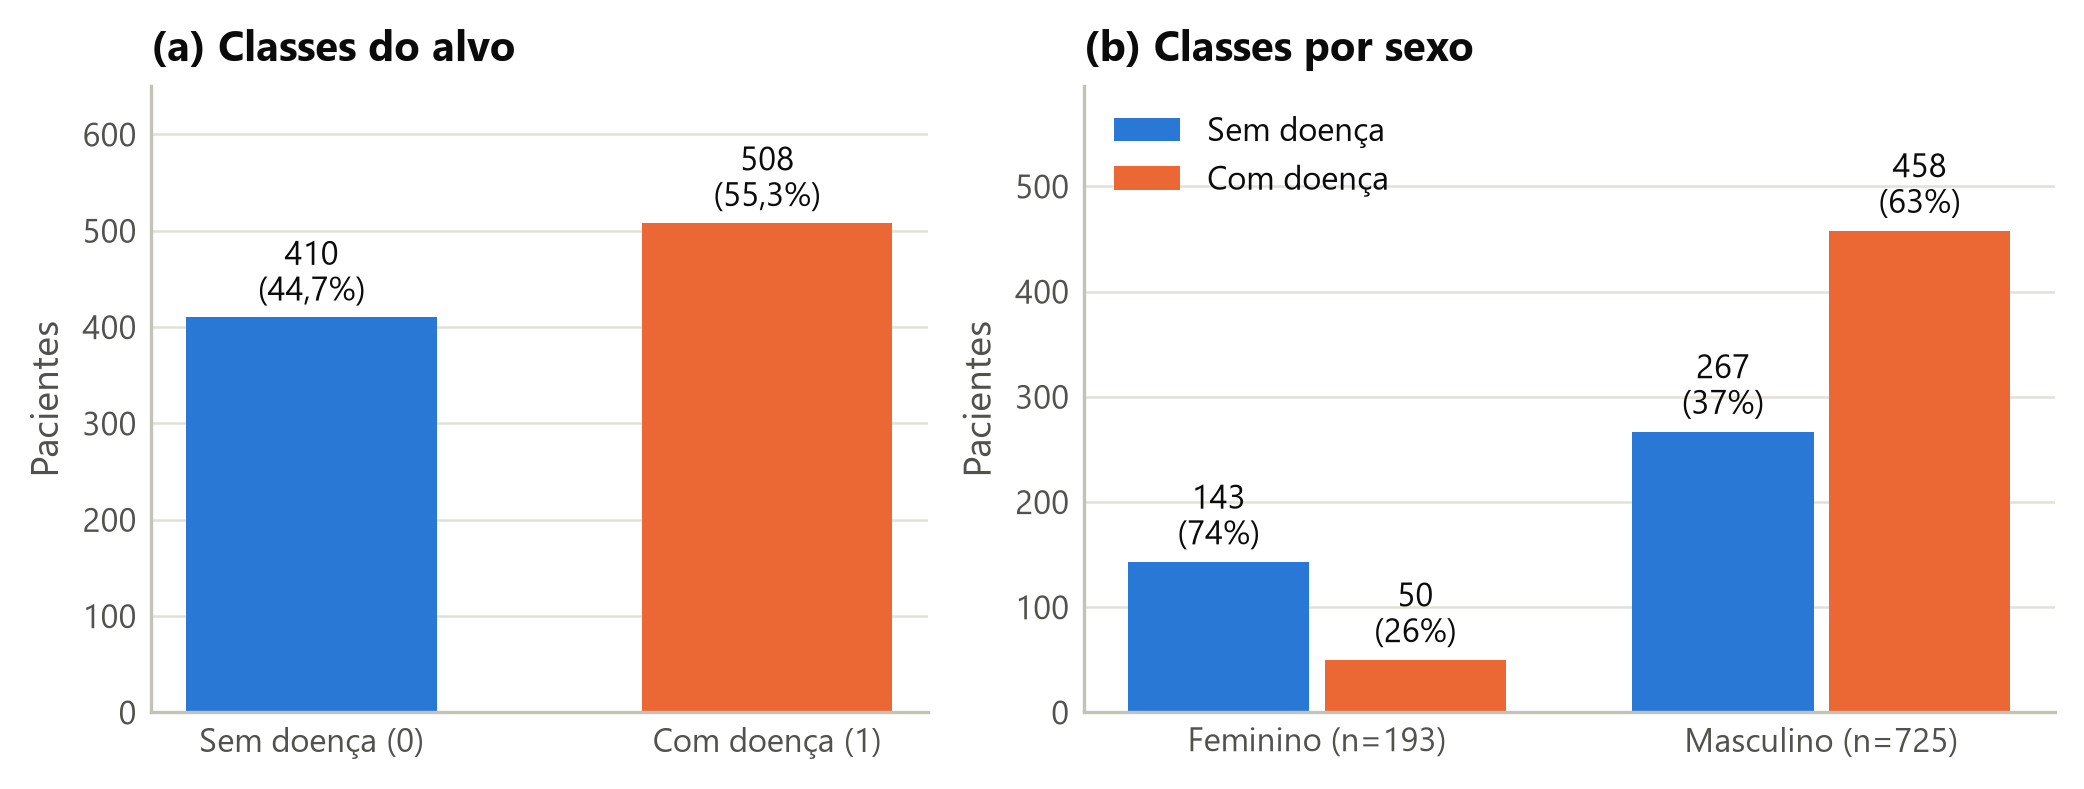
\includegraphics[width=.6\textwidth]{fig01_distribuicao_alvo.png}
\caption{Distribuição da variável-alvo: (a) no conjunto completo; (b) por sexo.}
\label{fig:alvo}
\end{figure}

A base não contém valores ausentes explícitos nem linhas duplicadas.
Contém, contudo, valores impossíveis: \texttt{Cholesterol} vale
zero em 172 registros (18,7\%) e \texttt{RestingBP}, em um, o que indica um
código de exame não medido. Essa ausência não é aleatória. A
Figura~\ref{fig:colesterol} mostra que 88\% dos pacientes sem colesterol
medido têm doença cardíaca, contra 48\% dos demais, de modo que a falta do
exame está associada ao alvo e, provavelmente, à base de origem do registro.
Quanto aos \textit{outliers}, pelo critério do intervalo interquartil e
desconsiderados os zeros, há 23 valores extremos em \texttt{Cholesterol}, 27
em \texttt{RestingBP} e 16 em \texttt{Oldpeak}, todos clinicamente plausíveis
e, por isso, mantidos.

\begin{figure}[!htb]
\centering
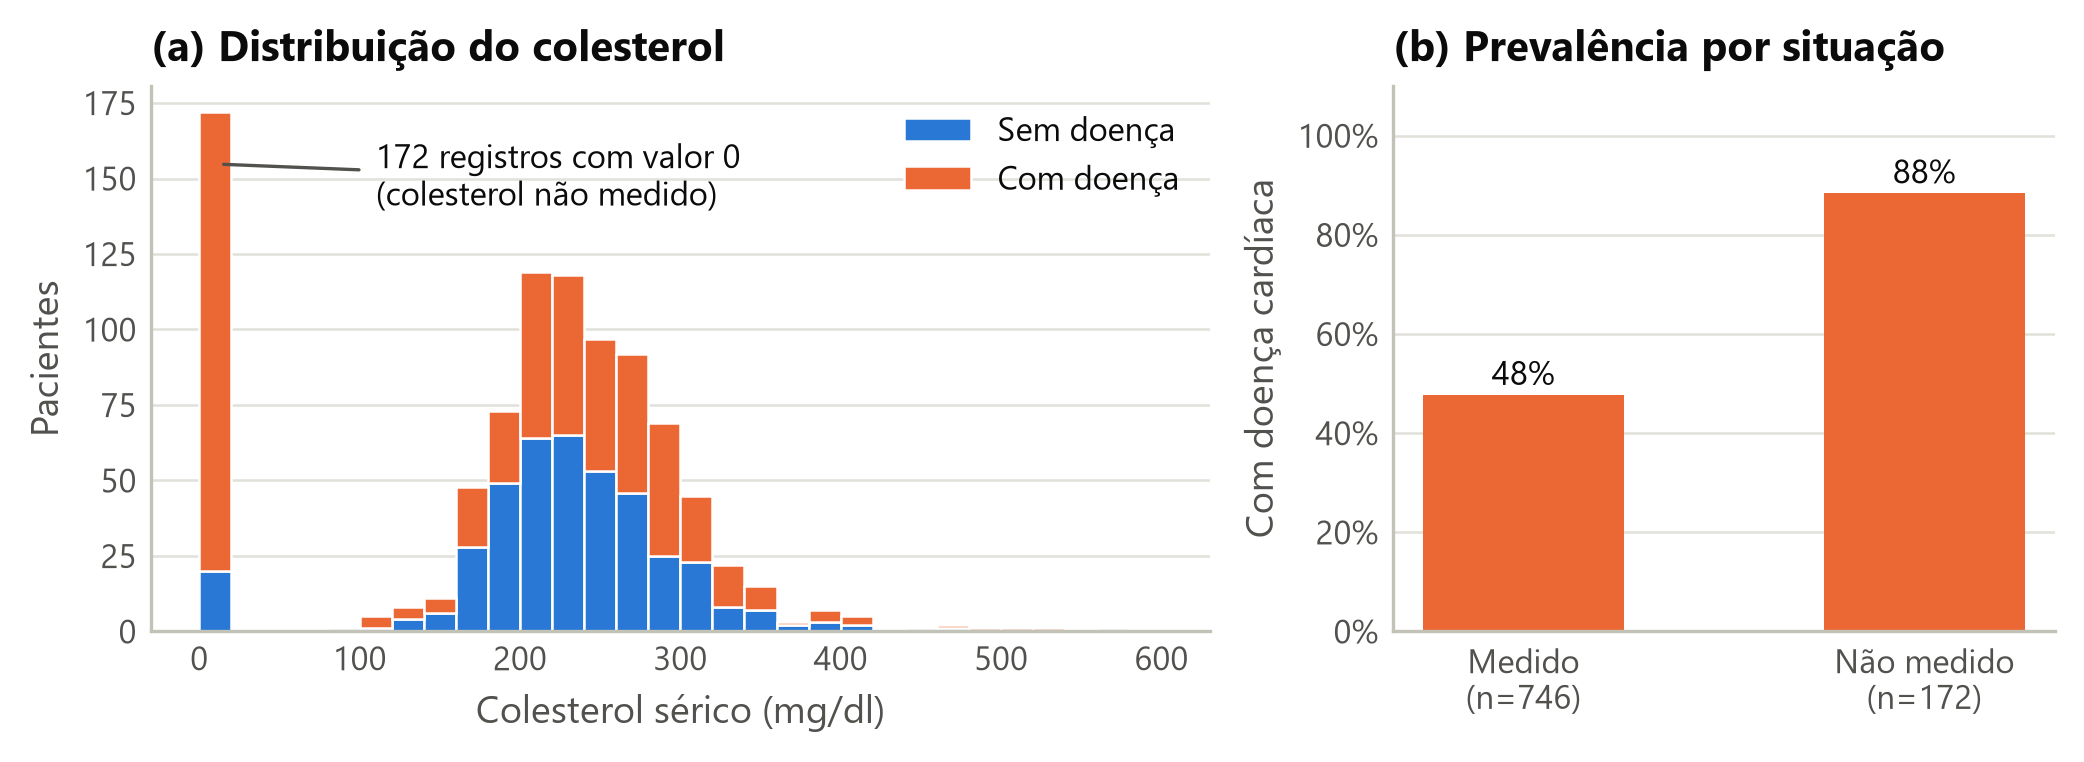
\includegraphics[width=.6\textwidth]{fig05_colesterol_ausente.png}
\caption{Colesterol sérico: (a) histograma com o pico em zero; (b) proporção de
pacientes com doença cardíaca conforme o exame foi ou não medido.}
\label{fig:colesterol}
\end{figure}

Entre os atributos numéricos, as maiores correlações de Spearman com o alvo
são as de \texttt{MaxHR} ($-0{,}41$) e \texttt{Oldpeak} ($0{,}39$), e a
maior correlação entre atributos é de $0{,}38$ em módulo, sem redundância
que justifique excluir colunas. Os atributos categóricos separam melhor as
classes: a doença aparece em 83\% dos pacientes com \texttt{ST\_Slope} plano
e em 18\% dos com inclinação ascendente. Como nenhum atributo é derivado do
diagnóstico, não há indício de vazamento do alvo.

\subsection{Pré-processamento}

A etapa de pré-processamento tem como objetivo adequar os dados aos modelos
a partir dos achados da análise exploratória. Em \texttt{Cholesterol} e
\texttt{RestingBP}, o zero é tratado como ausente e substituído pela
mediana. Não se cria uma coluna indicadora de ausência, visto que ela
ensinaria ao modelo um artefato de coleta; o efeito dessa decisão é medido
em um experimento de sensibilidade. Em seguida, os atributos numéricos são
padronizados, e os categóricos, codificados por \textit{one-hot}. Como o
desbalanceamento é leve, não se aplica reamostragem, e o uso de pesos de
classe é incluído na busca de hiperparâmetros.

Todas as transformações são reunidas em um único \texttt{Pipeline}, junto
com o classificador. Dessa forma, as estatísticas de imputação e de
padronização são ajustadas somente nos dados de treino e, na validação
cruzada, somente nas dobras de treino, o que evita o vazamento de dados.

\subsection{Treinamento e seleção dos modelos}

Inicialmente, os dados são divididos, de forma estratificada, em treino
(734 pacientes, 80\%) e teste (184 pacientes, 20\%), antes de qualquer
ajuste. São comparadas sete abordagens: a classe majoritária, como
\textit{baseline} trivial; a regressão logística, como \textit{baseline}
simples; e cinco modelos de famílias distintas. Para cada modelo, realiza-se
uma busca exaustiva em grade sobre o conjunto de treino, com validação
cruzada estratificada de 5 dobras repetida 3 vezes, o que resulta em 15
estimativas por configuração. A Tabela~\ref{tab:grades} apresenta o espaço de
busca e as configurações escolhidas; as grades completas, com as 303
configurações avaliadas, estão no repositório.

\begin{table}[!htb]
\centering
\caption{Espaço de busca de hiperparâmetros, configuração escolhida e número
de configurações avaliadas por modelo.}
\label{tab:grades}
\footnotesize\setlength{\tabcolsep}{4pt}
\begin{tabular}{@{}lp{6.9cm}p{3.9cm}r@{}}
\toprule
Modelo & Hiperparâmetros (faixa de busca) & Escolhido & Config. \\
\midrule
Reg. logística & $C$ (0,01 a 100); pesos de classe & $C{=}1$; balanceado & 16 \\
k-NN & $k$ (3 a 41); ponderação; métrica & $k{=}41$; distância; Manhattan & 36 \\
SVM (RBF) & $C$ (0,1 a 100); $\gamma$ (0,003 a 0,3); pesos de classe & $C{=}100$; $\gamma{=}0{,}003$; balanceado & 84 \\
Random Forest & árvores (300, 600); profundidade (4 a 12, $\infty$); mín. por folha (1 a 8); atributos por divisão & 600; 8; 4; $\sqrt{p}$ & 80 \\
Grad. Boosting & árvores (100 a 400); taxa (0,01 a 0,1); profundidade (2 a 4); subamostra (0,7; 1,0) & 400; 0,01; 3; 0,7 & 54 \\
MLP & camadas (8 a 32 neurônios); $\alpha$ ($10^{-4}$ a 1); taxa inicial & (8); $\alpha{=}1$; $10^{-3}$ & 32 \\
\bottomrule
\end{tabular}
\end{table}

O modelo final é definido como aquele de maior AUC-ROC média na validação
cruzada, regra fixada antes da consulta ao teste. Em seguida, o limiar de
decisão desse modelo é escolhido pelo máximo de $F_2$ nas predições
\textit{out-of-fold} do treino.

\subsection{Avaliação e interpretação}

Todos os modelos são avaliados uma única vez no conjunto de teste, por meio
de acurácia, precisão, revocação, F1, AUC-ROC e matriz de confusão. Para o
modelo final, estimam-se intervalos de confiança de 95\% por
\textit{bootstrap}, com 2.000 reamostragens. As diferenças de AUC na
validação cruzada são verificadas com o teste $t$ reamostrado corrigido de
\cite{nadeau:03}, que desconta a dependência entre as dobras. Para a
interpretação, calculam-se a importância por permutação e os valores SHAP
sobre os atributos originais, e analisam-se os erros e os subgrupos.

\section{Resultados e discussão}
\label{sec:resultados}

Esta seção apresenta e discute os resultados obtidos em cada avaliação.

\subsection{Comparação dos modelos}

A Tabela~\ref{tab:cv} apresenta os resultados da validação cruzada no treino.
Todos os modelos treinados superaram a classe majoritária, cuja revocação de
1,000 é trivial e vem acompanhada de AUC de 0,500. O Random Forest obteve a
maior AUC-ROC média (0,930), seguido de perto por Gradient Boosting (0,928) e
MLP (0,927). Essas diferenças, contudo, são pequenas diante do desvio-padrão
entre dobras, de cerca de 0,025. O teste $t$ corrigido não rejeitou a igualdade entre o Random Forest e
nenhum outro modelo treinado ao nível de 5\%: o menor $p$-valor foi o da
comparação com a regressão logística (diferença de 0,010; $p = 0{,}053$).

\begin{table}[!htb]
\centering
\caption{Validação cruzada estratificada 5$\times$3 no treino: média $\pm$
desvio-padrão da melhor configuração de cada modelo. Em negrito, o melhor valor
entre os modelos treinados.}
\label{tab:cv}
\footnotesize
\begin{tabular}{@{}lcccc@{}}
\toprule
Modelo & Precisão & Revocação & F1 & AUC-ROC \\
\midrule
Classe majoritária & 0,553 $\pm$ 0,003 & 1,000 $\pm$ 0,000 & 0,712 $\pm$ 0,002 & 0,500 $\pm$ 0,000 \\
Regressão logística & 0,863 $\pm$ 0,035 & 0,844 $\pm$ 0,030 & 0,852 $\pm$ 0,022 & 0,920 $\pm$ 0,027 \\
k-NN & 0,857 $\pm$ 0,044 & 0,889 $\pm$ 0,018 & 0,872 $\pm$ 0,024 & 0,922 $\pm$ 0,029 \\
SVM (RBF) & \textbf{0,865} $\pm$ 0,033 & 0,856 $\pm$ 0,029 & 0,860 $\pm$ 0,019 & 0,922 $\pm$ 0,027 \\
Random Forest & 0,853 $\pm$ 0,039 & \textbf{0,901} $\pm$ 0,029 & \textbf{0,876} $\pm$ 0,024 & \textbf{0,930} $\pm$ 0,024 \\
Gradient Boosting & 0,858 $\pm$ 0,038 & 0,883 $\pm$ 0,034 & 0,869 $\pm$ 0,022 & 0,928 $\pm$ 0,024 \\
MLP & 0,849 $\pm$ 0,038 & 0,884 $\pm$ 0,034 & 0,866 $\pm$ 0,026 & 0,927 $\pm$ 0,024 \\
\bottomrule
\end{tabular}
\end{table}

Pela regra fixada na metodologia, o Random Forest foi definido como modelo
final. A Tabela~\ref{tab:teste} e a Figura~\ref{fig:roc} apresentam o
desempenho no conjunto de teste, com limiar 0,50. Analisando a
Tabela~\ref{tab:teste}, percebe-se que as AUC no teste, entre 0,923 e 0,938,
confirmam as estimativas da validação cruzada, o que indica que o protocolo
não superestimou o desempenho. Observa-se também que a ordem dos modelos se
alterou: no teste, k-NN e Gradient Boosting obtiveram os melhores valores, e
o Random Forest ficou em último entre os modelos treinados. O intervalo de
confiança de 95\% da AUC do Random Forest, de 0,879 a 0,959, contém a AUC de
todos os outros modelos. Assim, com 184 pacientes de teste, os seis modelos
são estatisticamente indistinguíveis. Como a troca do modelo com base no
teste invalidaria o teste como estimativa imparcial, a escolha feita no
treino foi mantida. Verifica-se ainda que o \textit{baseline} linear captura
quase toda a estrutura dos dados, pois a regressão logística ficou a 0,010
de AUC do melhor modelo na validação cruzada.

\begin{table}[!htb]
\centering
\caption{Desempenho no conjunto de teste (184 pacientes). Em negrito, o melhor
valor entre os modelos treinados com limiar 0,50. A última linha usa o limiar
escolhido no treino.}
\label{tab:teste}
\footnotesize
\begin{tabular}{@{}lccccc@{}}
\toprule
Modelo & Acurácia & Precisão & Revocação & F1 & AUC-ROC \\
\midrule
Classe majoritária & 0,554 & 0,554 & 1,000 & 0,713 & 0,500 \\
Regressão logística & 0,875 & 0,899 & 0,873 & 0,886 & 0,931 \\
k-NN & \textbf{0,891} & \textbf{0,902} & \textbf{0,902} & \textbf{0,902} & \textbf{0,938} \\
SVM (RBF) & 0,880 & 0,885 & \textbf{0,902} & 0,893 & 0,936 \\
Random Forest & 0,848 & 0,849 & 0,882 & 0,865 & 0,923 \\
Gradient Boosting & \textbf{0,891} & \textbf{0,902} & \textbf{0,902} & \textbf{0,902} & 0,931 \\
MLP & 0,870 & 0,875 & 0,892 & 0,883 & 0,930 \\
\midrule
Random Forest, limiar 0,29 & 0,826 & 0,782 & 0,951 & 0,858 & 0,923 \\
\bottomrule
\end{tabular}
\end{table}

\begin{figure}[!htb]
\centering
\begin{minipage}[c]{.42\textwidth}
\centering
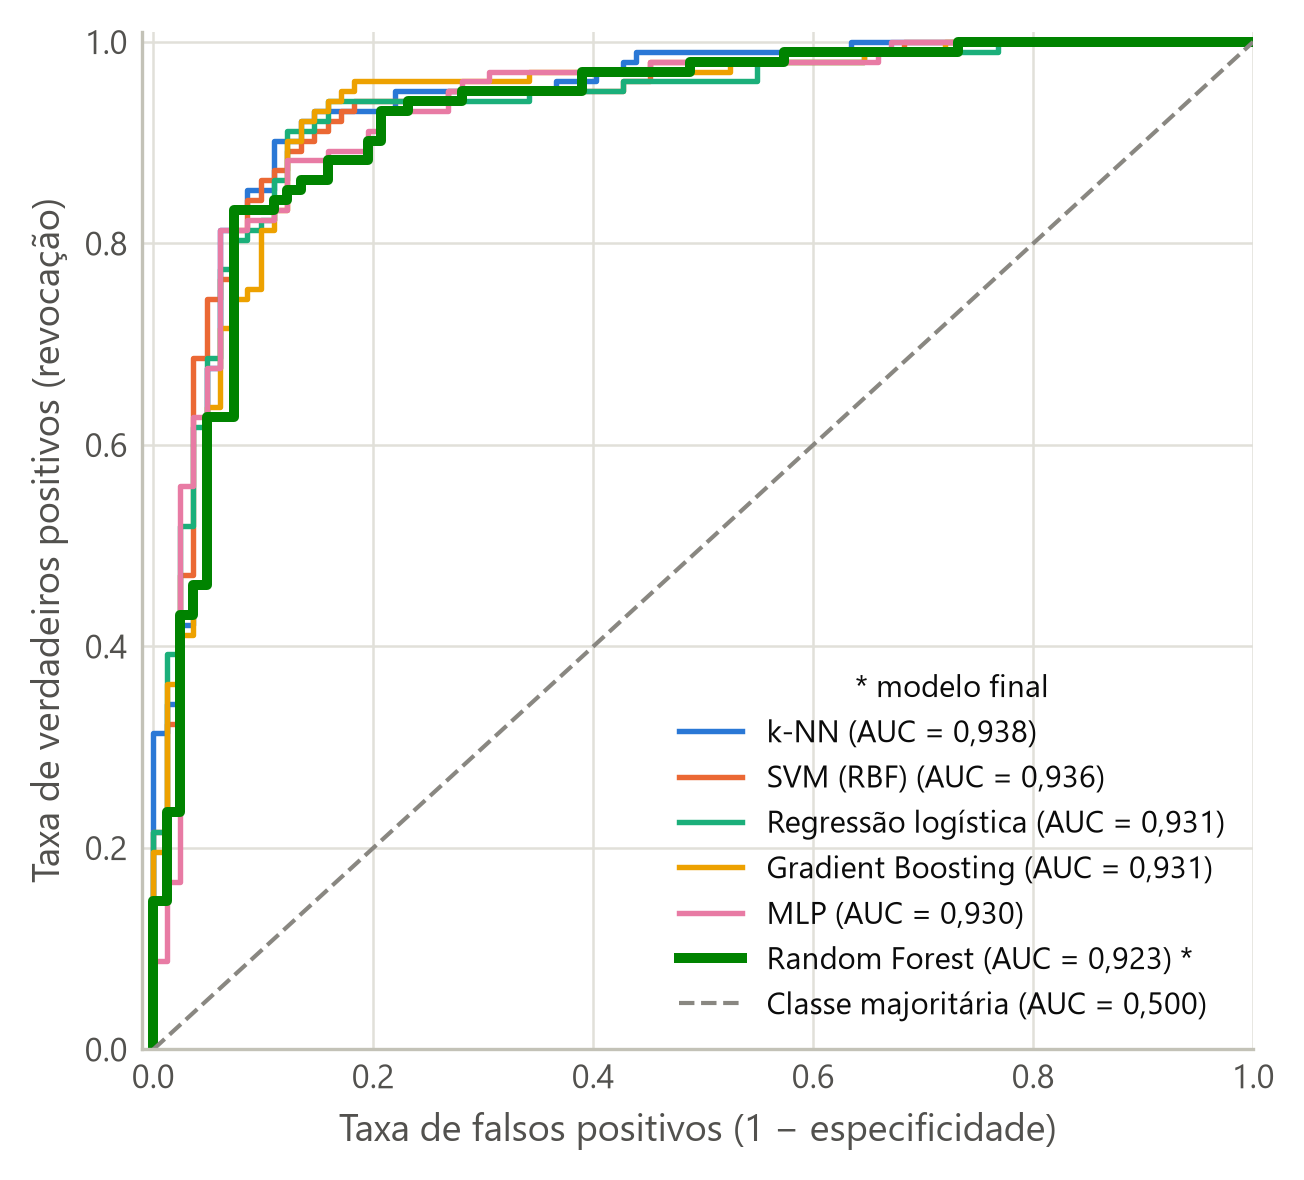
\includegraphics[width=\textwidth]{fig06_curvas_roc.png}
\end{minipage}\hfill
\begin{minipage}[c]{.54\textwidth}
\centering
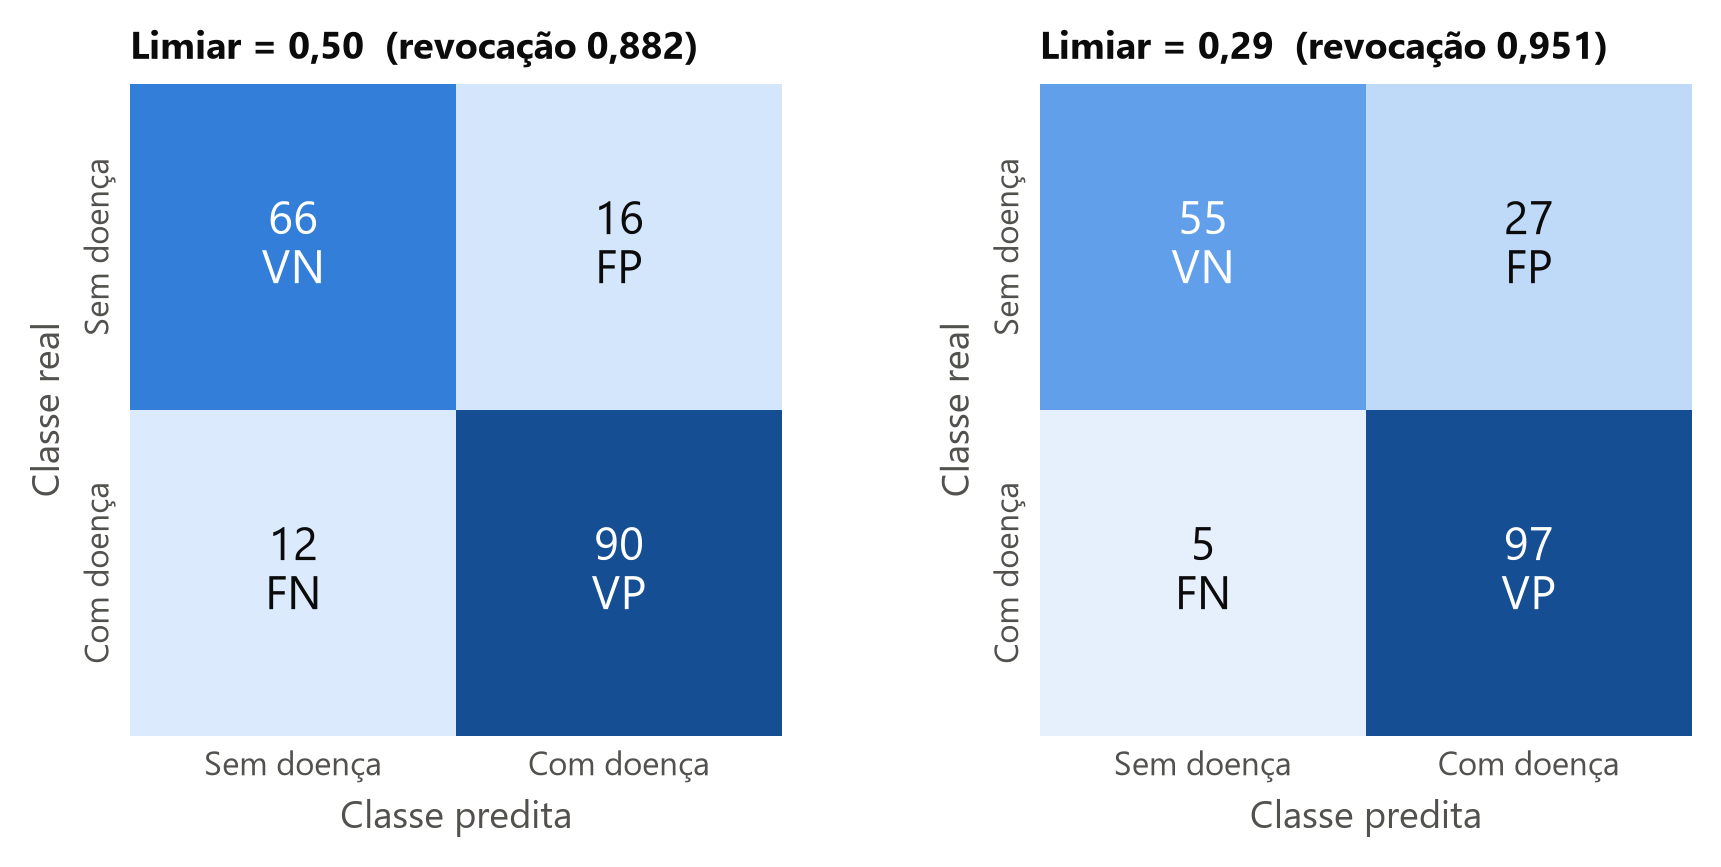
\includegraphics[width=\textwidth]{fig07_matriz_confusao.png}
\end{minipage}
\caption{À esquerda, curvas ROC no conjunto de teste. À direita, matrizes de
confusão do modelo final no teste com limiar 0,50 e com o limiar escolhido
(0,29).}
\label{fig:roc}
\end{figure}

No experimento de sensibilidade, a inclusão de um indicador de colesterol
ausente elevou a AUC média na validação cruzada de 0,930 para 0,932 no Random
Forest e de 0,920 para 0,926 na regressão logística. Esse ganho é menor do
que o desvio-padrão entre dobras, de modo que a decisão de não utilizar o
indicador custou pouco.

Em relação à literatura, a AUC de 0,923 é inferior à de 0,97 reportada por
\cite{chulde:25}, e as acurácias obtidas, entre 0,848 e 0,891, situam-se
próximas às de \cite{amin:19} e \cite{mohan:19}. Essa comparação é apenas
indicativa, visto que as divisões dos dados e o tratamento dos valores
ausentes diferem entre os trabalhos.

\subsection{Limiar de decisão do modelo final}

Com limiar 0,50, o Random Forest deixou de identificar 12 dos 102 doentes do
teste. Nas predições \textit{out-of-fold} do treino, $F_2$ foi máximo no
limiar 0,29, no qual a revocação foi de 0,978 e a precisão, de 0,796.
Aplicado ao teste, conforme a Figura~\ref{fig:roc}, esse limiar reduziu os
falsos negativos de 12 para 5 e elevou os falsos positivos de 16 para 27. A
revocação passou de 0,882 para 0,951 (IC 95\%: 0,907 a 0,990), a precisão
caiu de 0,849 para 0,782 (IC 95\%: 0,708 a 0,854) e a especificidade ficou em
0,671. Para uma ferramenta de triagem, essa troca é a desejada, embora um em
cada três pacientes saudáveis passe a ser sinalizado. O limiar constitui,
portanto, um parâmetro de política de uso, a ser revisto conforme a
capacidade de atendimento do serviço.

\subsection{Interpretação do modelo}

A Figura~\ref{fig:importancia} apresenta duas medidas de importância
calculadas no teste. Ambas concordam nos dois primeiros lugares: a inclinação
do segmento ST no esforço (\texttt{ST\_Slope}) foi o atributo mais utilizado,
com queda de 0,127 na AUC ao ser embaralhada, seguida do tipo de dor no peito
(0,038). Na sequência, aparecem sexo, \texttt{Oldpeak} e angina no esforço.
Colesterol, pressão arterial e ECG de repouso contribuíram pouco, e a idade
apresentou importância por permutação praticamente nula, embora se
correlacione com o alvo, o que sugere que sua informação já está nos
resultados do teste de esforço. Esse padrão é clinicamente coerente e indica
também que o modelo só é útil para pacientes que realizaram teste de esforço.

\begin{figure}[!htb]
\centering
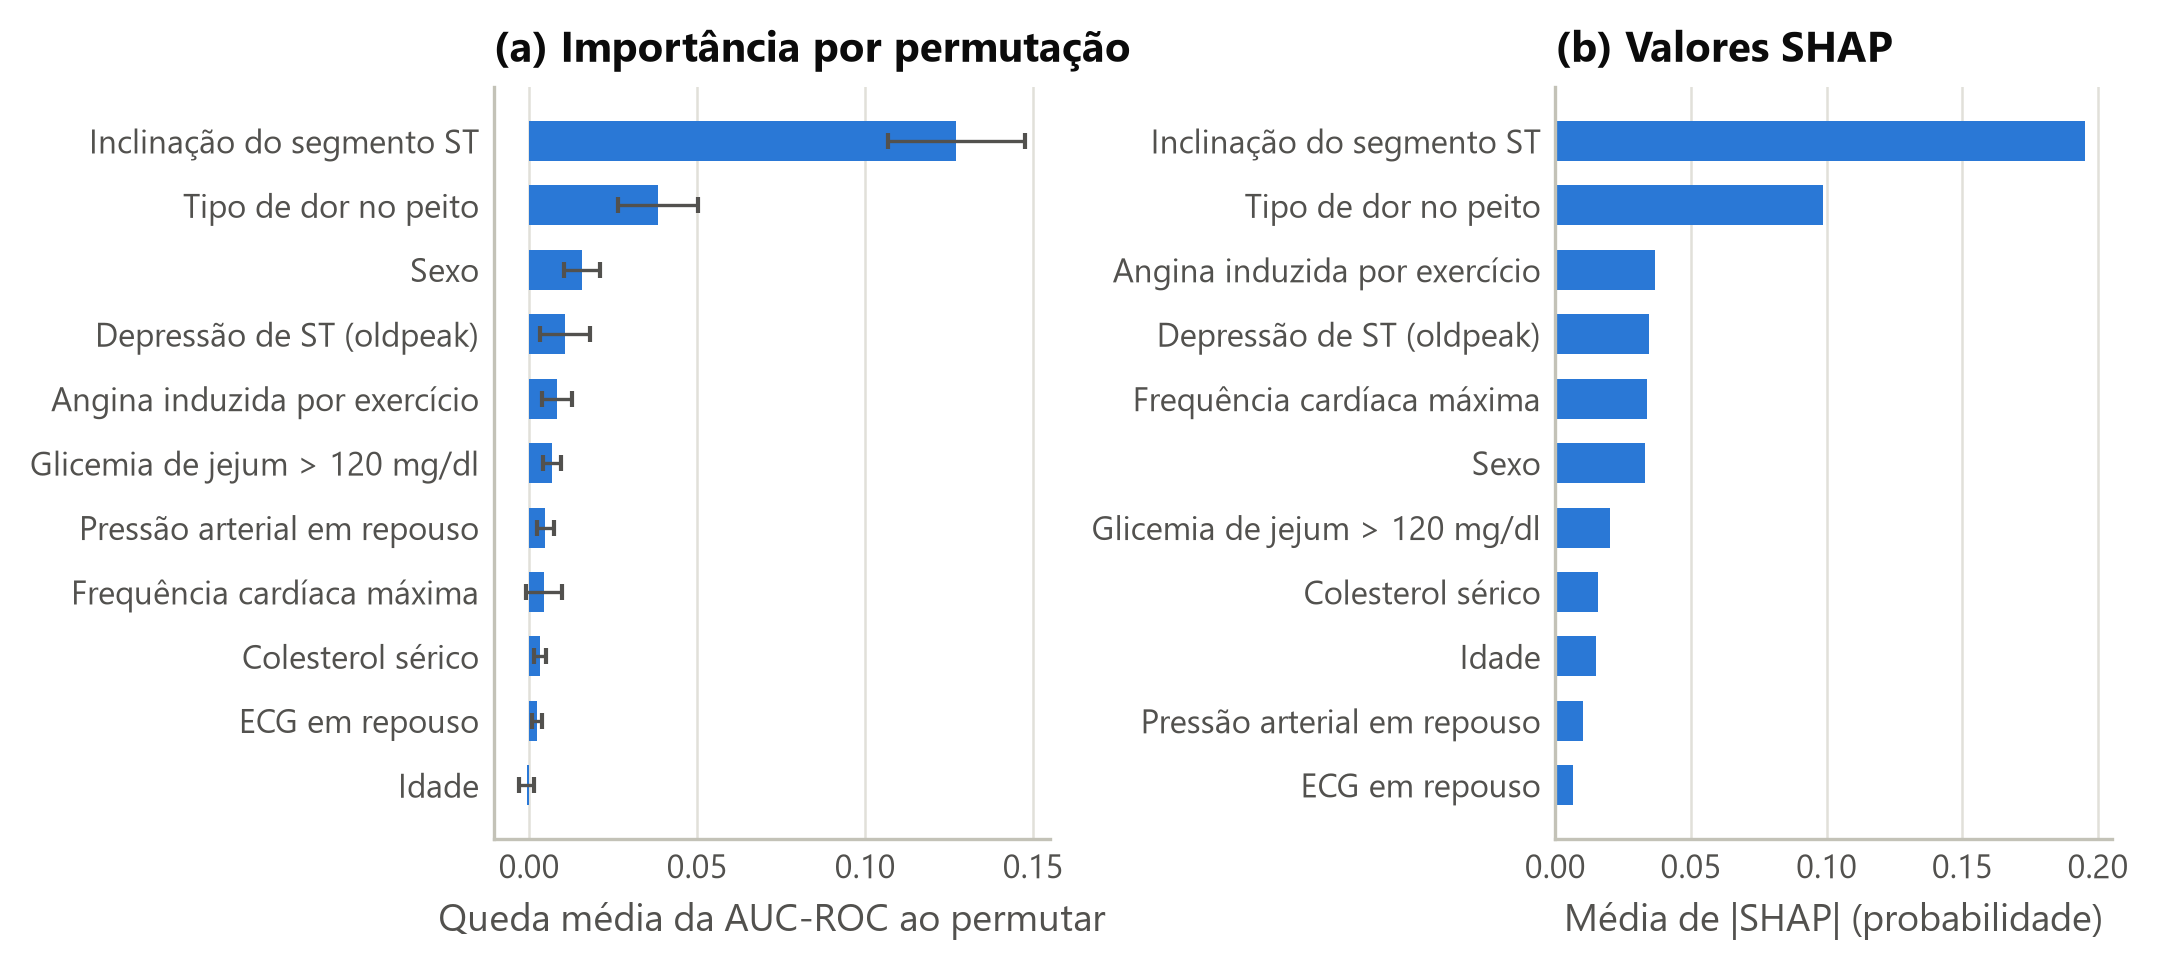
\includegraphics[width=.72\textwidth]{fig09_importancia_atributos.png}
\caption{Importância dos atributos no conjunto de teste: (a) queda média da
AUC-ROC em 50 permutações, com desvio-padrão; (b) média do valor absoluto dos
valores SHAP.}
\label{fig:importancia}
\end{figure}

\subsection{Análise de erros e de subgrupos}

Os cinco falsos negativos do teste apresentaram o mesmo perfil: todos são
homens com \texttt{ST\_Slope} ascendente, sem angina no esforço, com dor no
peito de tipo não assintomático e frequência cardíaca máxima elevada (média
de 172 bpm, contra 128 bpm entre os verdadeiros positivos). Trata-se de
doentes cujo teste de esforço tem aparência normal. Os 27 falsos positivos,
por sua vez, assemelham-se aos doentes: 56\% têm \texttt{ST\_Slope} plano e
44\% são assintomáticos, contra 2\% e 11\% entre os verdadeiros negativos.

A Tabela~\ref{tab:subgrupos} detalha o desempenho por subgrupo. Entre as
mulheres, o modelo identificou os 6 casos de doença, mas sinalizou 11 das 32
saudáveis, e a precisão caiu para 0,353. Como a prevalência nesse grupo é
baixa (16\%), o limiar único gera proporcionalmente mais alarmes falsos.
Entre os pacientes sem colesterol medido, a AUC caiu para 0,698 e a
especificidade, para 0,286. Esses dois subgrupos são pequenos (38 e 43
pacientes), o que confere grande incerteza aos valores, mas eles apontam
onde o modelo é menos confiável.

\begin{table}[!htb]
\centering
\caption{Modelo final no teste, por subgrupo, com limiar 0,29.}
\label{tab:subgrupos}
\footnotesize\setlength{\tabcolsep}{4.5pt}
\begin{tabular}{@{}lrrccccrr@{}}
\toprule
Subgrupo & $n$ & Doentes & Precisão & Revocação & Especif. & AUC & FN & FP \\
\midrule
Todos & 184 & 102 & 0,782 & 0,951 & 0,671 & 0,923 & 5 & 27 \\
Homens & 146 & 96 & 0,850 & 0,948 & 0,680 & 0,903 & 5 & 16 \\
Mulheres & 38 & 6 & 0,353 & 1,000 & 0,656 & 0,953 & 0 & 11 \\
Colesterol medido & 141 & 66 & 0,738 & 0,939 & 0,707 & 0,936 & 4 & 22 \\
Colesterol não medido & 43 & 36 & 0,875 & 0,972 & 0,286 & 0,698 & 1 & 5 \\
\bottomrule
\end{tabular}
\end{table}

\section{A aplicação}
\label{sec:aplicacao}

Esta seção apresenta a aplicação desenvolvida para disponibilizar o modelo a
profissionais e estudantes de saúde. A aplicação é construída como uma
página web com a biblioteca Streamlit, e sua arquitetura é apresentada na
Figura~\ref{fig:arquitetura}. O treinamento grava três artefatos: o
\texttt{Pipeline} completo, em formato \texttt{joblib}; um arquivo de
metadados com o limiar e as métricas; e uma amostra de 50 pacientes de
treino, utilizada como referência para os valores SHAP. A aplicação carrega
esses arquivos e não reimplementa nenhuma etapa de pré-processamento: os
valores informados são validados e entregues ao \texttt{Pipeline} salvo.

\begin{figure}[!htb]
\centering
\scriptsize
\begin{tikzpicture}[
  node distance=4mm and 7mm,
  box/.style={draw, rounded corners=2pt, align=center, inner sep=3pt, minimum height=8mm, text width=2.75cm},
  file/.style={box, fill=black!6},
  arr/.style={-{Stealth[length=2mm]}, thick}]
\node[file] (csv) {heart.csv\\(918 pacientes)};
\node[box, right=of csv] (train) {src/train.py\\busca em grade e validação cruzada};
\node[file, right=of train] (model) {modelo\_final.joblib\\metadata.json\\shap\_background.csv};
\node[box, below=7mm of model] (service) {app/service.py\\carrega o pipeline, prediz e explica};
\node[box, left=of service] (valid) {app/validation.py\\tipos, faixas e categorias};
\node[box, left=of valid] (ui) {Interface Streamlit\\formulário ou CSV};
\node[file, below=5mm of service] (logs) {logs/predicoes.csv\\logs/feedback.csv};
\node[box, below=5mm of ui] (out) {Probabilidade, classe e contribuição SHAP};
\draw[arr] (csv) -- (train);
\draw[arr] (train) -- (model);
\draw[arr] (model) -- (service);
\draw[arr] (ui) -- (valid);
\draw[arr] (valid) -- (service);
\draw[arr] (service) -- (logs);
\draw[arr] (service.south west) -- (out.north east);
\node[above=1mm of train, font=\scriptsize\itshape] {treino (executado uma vez)};
\node[below=1mm of valid, font=\scriptsize\itshape] {uso (a cada predição)};
\end{tikzpicture}
\caption{Arquitetura: o treino produz os artefatos que a aplicação carrega.}
\label{fig:arquitetura}
\end{figure}

A interface possui três abas. Na primeira, o usuário preenche um formulário
com os dados de um paciente (Figura~\ref{fig:telas}, à esquerda). Campos
vazios, valores fora das faixas de plausibilidade clínica e categorias
desconhecidas geram mensagens que indicam o campo a corrigir e a faixa
aceita. A saída (Figura~\ref{fig:telas}, à direita) apresenta a probabilidade
estimada, o limiar em uso, a classificação em risco baixo ou elevado e a
contribuição SHAP de cada atributo. A segunda aba recebe um arquivo CSV com
vários pacientes e devolve os resultados para \textit{download}, e a
terceira descreve os dados, o protocolo e as métricas.

\begin{figure}[!htb]
\centering
\begin{minipage}[c]{.41\textwidth}
\centering
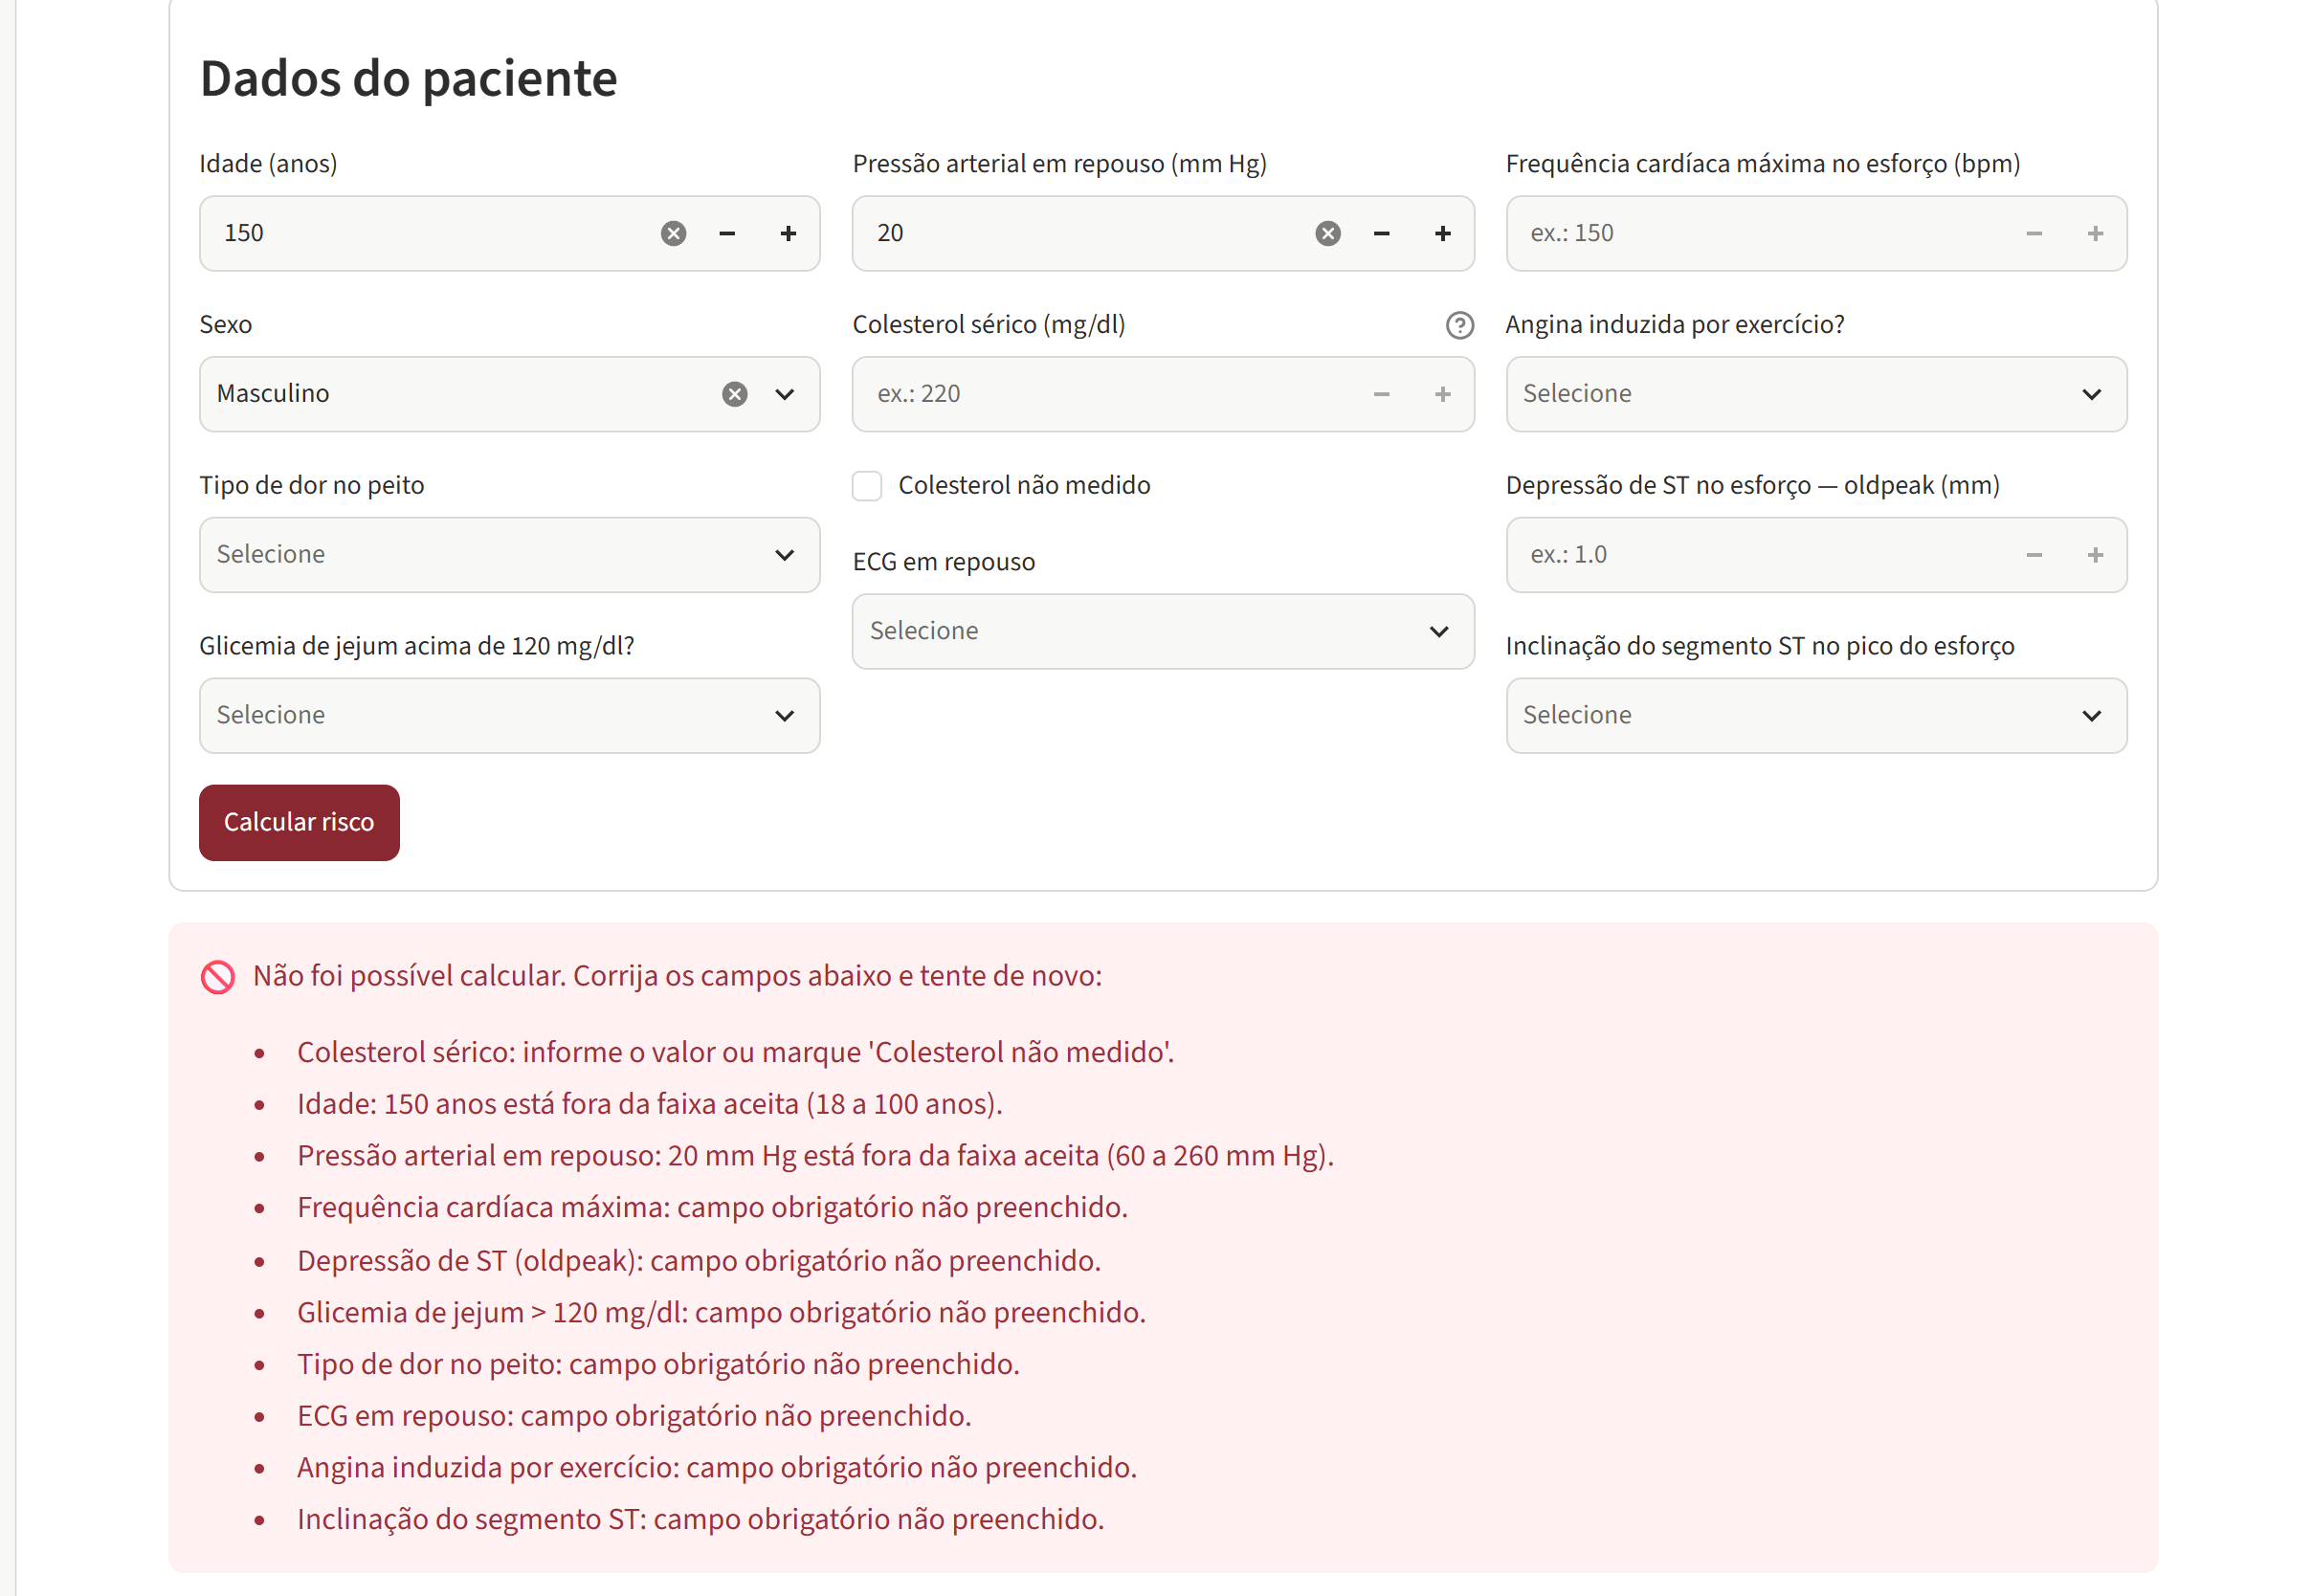
\includegraphics[width=\textwidth]{tela_erros.png}
\end{minipage}\hfill
\begin{minipage}[c]{.41\textwidth}
\centering
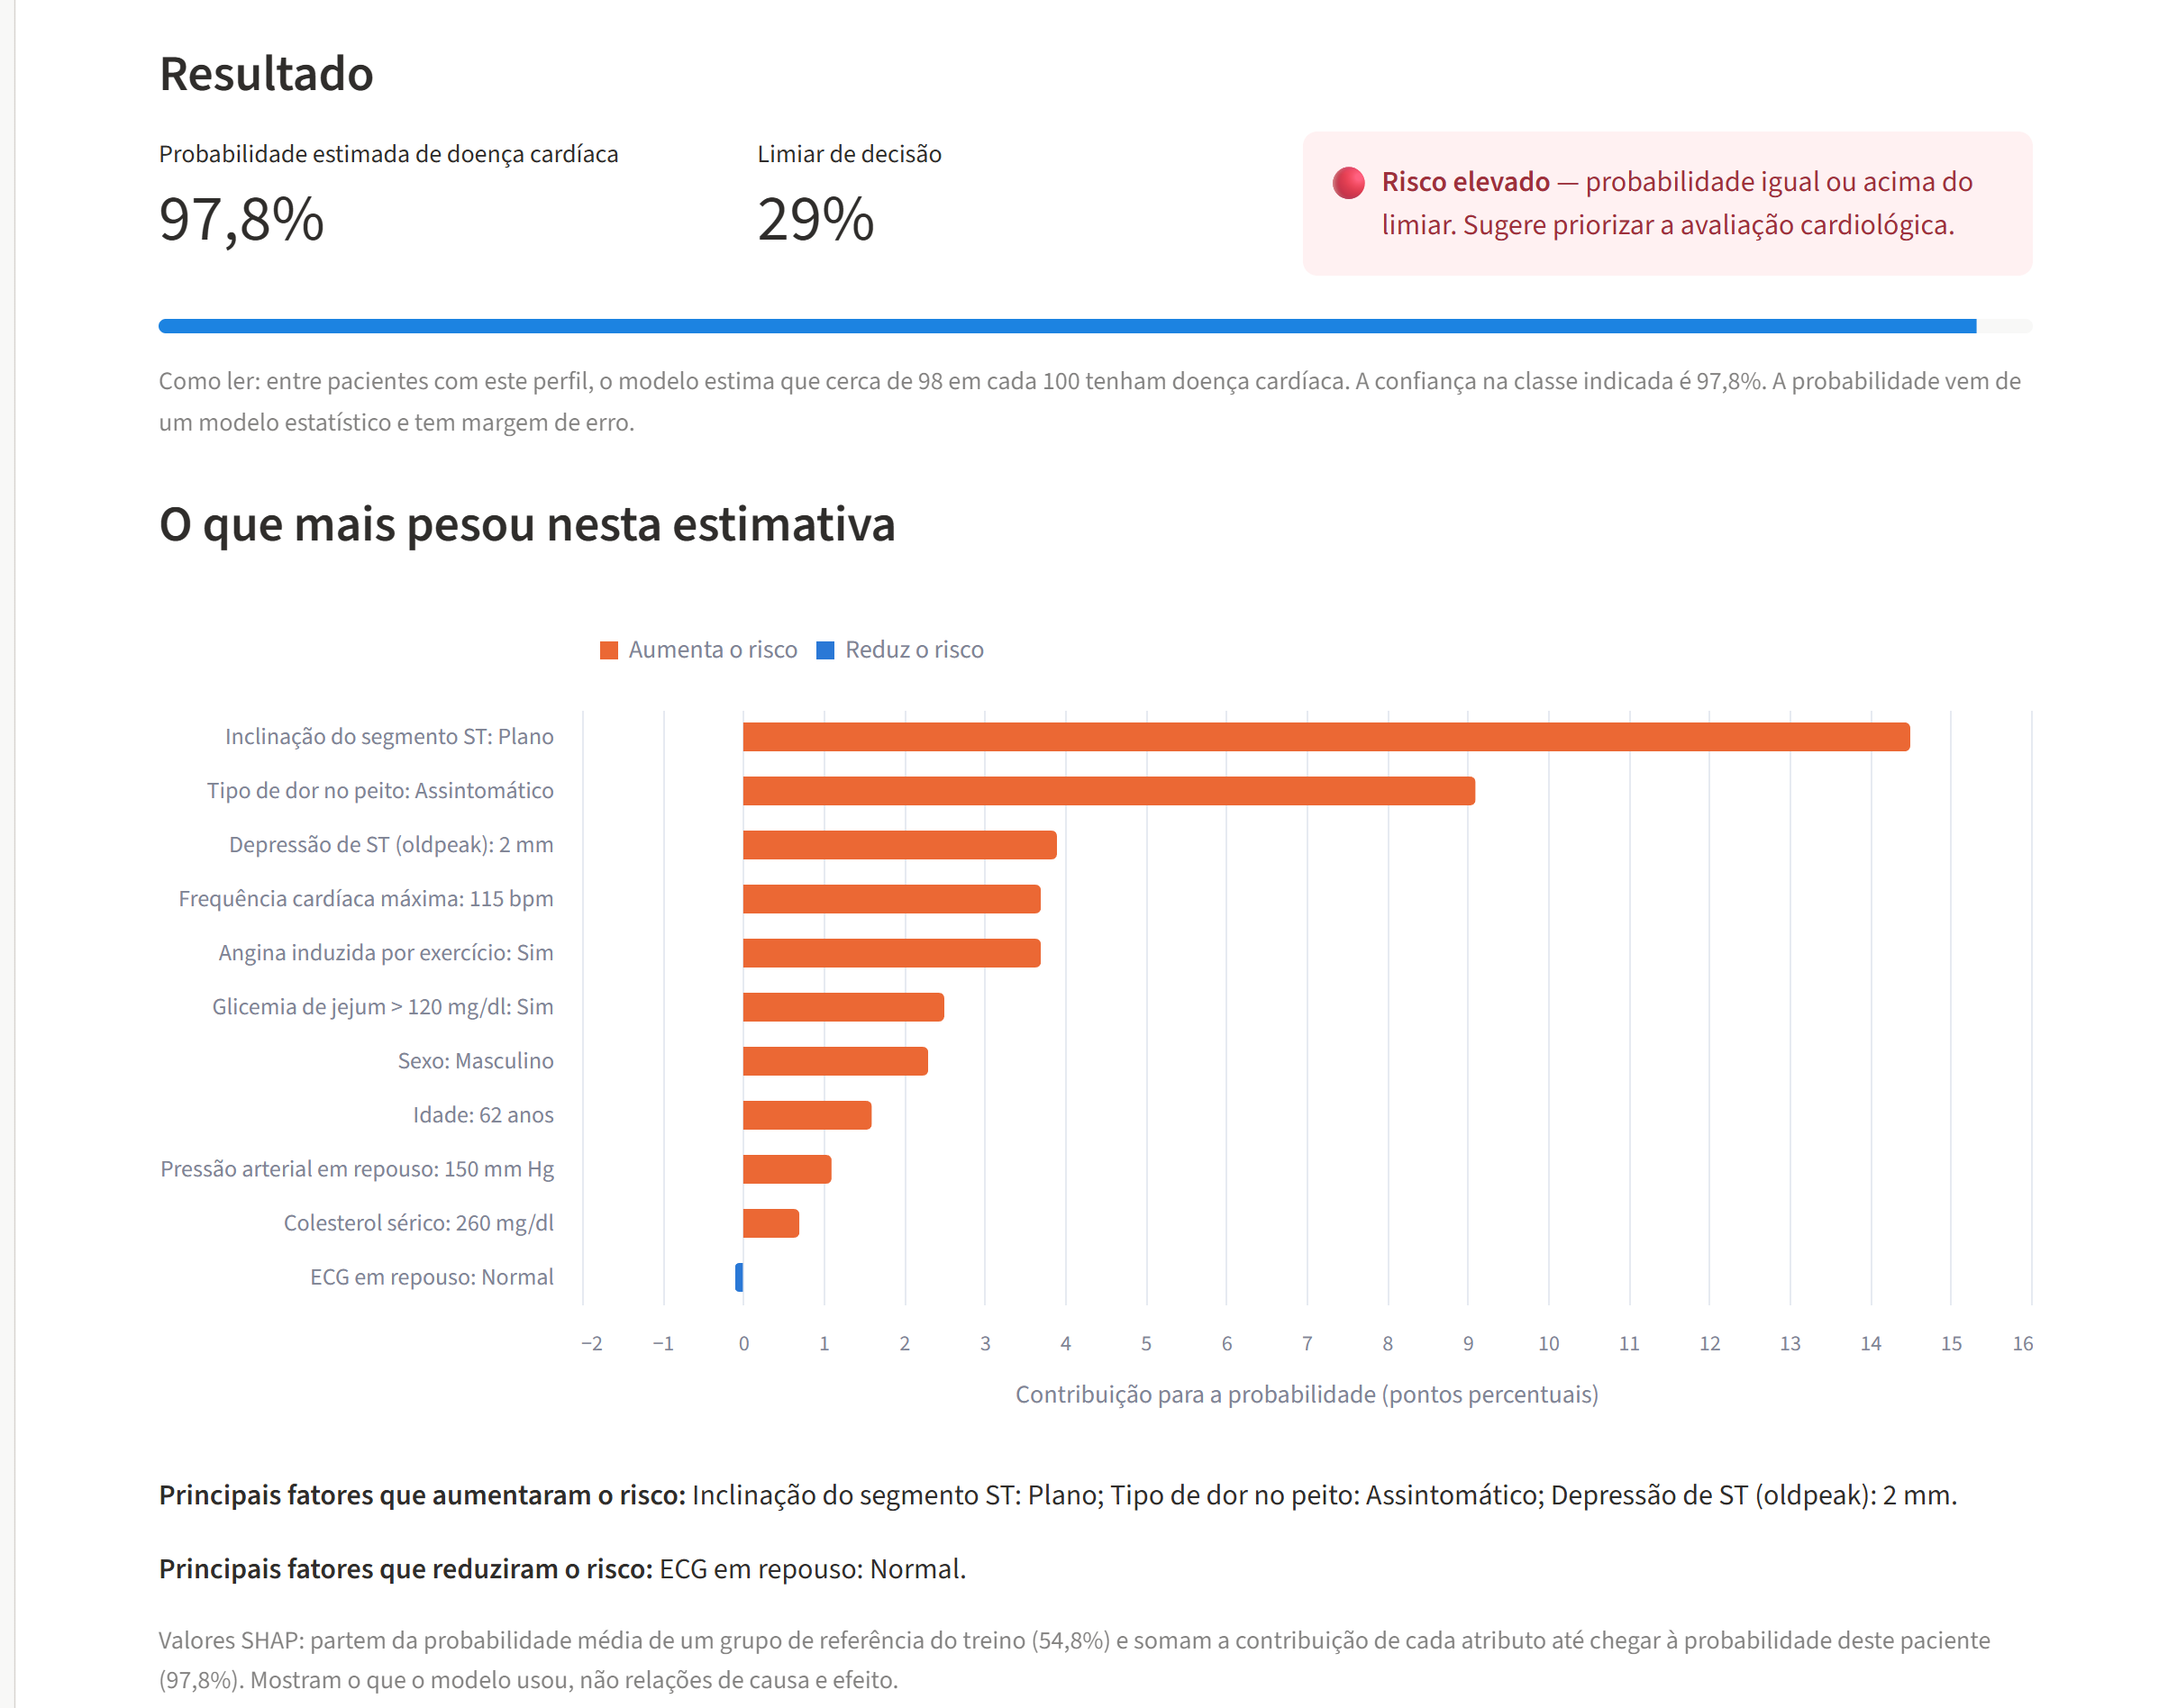
\includegraphics[width=\textwidth]{tela_resultado.png}
\end{minipage}
\caption{Aplicação em uso. À esquerda, formulário com entradas inválidas e as
mensagens de erro. À direita, resultado para um paciente: probabilidade,
classificação e contribuição de cada atributo.}
\label{fig:telas}
\end{figure}

O topo da página informa que a ferramenta não realiza diagnóstico nem
substitui a avaliação médica, e um painel descreve a quem ela se destina e
quais são suas limitações. Cada predição pode ser registrada em arquivo, sem
identificador do paciente, e o usuário pode avaliar a estimativa. O
repositório inclui ainda 42 testes automatizados, que verificam a ausência
de vazamento, a validação de entradas, o modelo salvo e a interface.

\section{Considerações éticas e limitações}
\label{sec:etica}

Quanto aos vieses, a base possui 79\% de homens, e o modelo gera
proporcionalmente mais alarmes falsos em mulheres
(Tabela~\ref{tab:subgrupos}). Não há informação de raça, renda ou acesso a
serviços de saúde, de modo que não é possível verificar disparidades como as
documentadas por \cite{obermeyer:19} em um algoritmo de saúde em uso real.

Quanto à generalização, os dados provêm de pacientes encaminhados para
investigação cardiológica nos Estados Unidos e na Europa, em sua maioria na
década de 1980, com prevalência de 55\%, muito acima da observada na atenção
básica. O modelo não foi validado em pacientes brasileiros nem em uso
prospectivo, e o alvo é a presença de doença cardíaca, não a ocorrência
futura de insuficiência cardíaca.

Quanto à privacidade, a base é pública e anonimizada, e a aplicação não
solicita nome nem documento. Dados de saúde, contudo, são sensíveis pela LGPD
\cite{lgpd:18}, e um uso real exigiria base legal e controle de acesso.
Quanto ao uso indevido, o principal risco é o emprego da ferramenta para
diagnóstico ou para negar atendimento a quem recebeu risco baixo, resultado
que não descarta a doença: 5 dos 102 doentes do teste foram assim
classificados.

\section{Conclusão e trabalhos futuros}
\label{sec:conclusao}

Este trabalho avaliou classificadores para a estimativa do risco de doença
cardíaca a partir de dados clínicos de rotina. Sob um protocolo sem vazamento
de dados, seis modelos de cinco famílias obtiveram AUC-ROC entre 0,923 e
0,938 no teste, todos muito acima do \textit{baseline} trivial e
estatisticamente indistinguíveis entre si. O Random Forest, selecionado pela
validação cruzada, identificou 95,1\% dos doentes com o limiar ajustado, ao
custo de sinalizar um terço dos saudáveis. Verificou-se que o modelo depende
sobretudo dos resultados do teste de esforço e falha em doentes cujo teste
tem aparência normal. O modelo foi integrado a uma aplicação que carrega o
\textit{pipeline} salvo, valida as entradas e explica cada predição.

Como trabalhos futuros, pretende-se validar o modelo em dados brasileiros
recentes, calibrar as probabilidades e definir limiares por subgrupo. Também
se pretende avaliar a substituição do Random Forest pela regressão logística,
de desempenho próximo e mais simples de auditar.

\section*{Declaração de uso de IA}

% TODO (autores): ajustar este texto para que descreva exatamente o uso feito pela equipe.
Foi utilizada a seguinte ferramenta de IA generativa na elaboração deste
trabalho:
\begin{itemize}
  \item \textbf{Claude} (Anthropic), por meio do Claude Code: utilizado na
  escrita e depuração do código de análise exploratória, treino, avaliação,
  aplicação e testes; na sugestão da estrutura das seções; e na redação e
  revisão do texto deste artigo.
\end{itemize}
Todos os resultados foram produzidos pela execução dos \textit{scripts} do
repositório sobre o conjunto de dados real, e as referências foram conferidas
nos registros de publicação. As análises e conclusões apresentadas são de
responsabilidade dos autores.

\bibliographystyle{sbc}
\bibliography{referencias}

\end{document}
